\documentclass{bioinfo}

\usepackage{url}
\usepackage{booktabs}
\usepackage{graphicx}

\copyrightyear{2026}
\pubyear{2026}

\begin{document}

\firstpage{1}

\subtitle{Application Note}

\title{ggwas: a comprehensive ggplot2 toolkit for genome-wide association study visualization}

\author[Czech]{Bartosz Czech\,$^{1,*}$}

\address{$^{1}$Department of Genetics, Wroc\l{}aw University of Environmental and Life Sciences, Wroc\l{}aw, Poland}

\corresp{$^\ast$To whom correspondence should be addressed.}

\history{Received on XXXXX; revised on XXXXX; accepted on XXXXX}

\editor{Associate Editor: XXXXX}

\abstract{
\textbf{Summary:} Genome-wide association studies (GWAS) are central to modern genetics, yet the R ecosystem lacks a unified, customizable visualization package that scales to biobank-era datasets. We present ggwas, a ggplot2-based R package providing 17 publication-ready plot types for GWAS summary statistics. Beyond standard Manhattan and QQ plots, ggwas offers novel visualizations including enrichment Manhattan plots with functional annotation overlays, multi-trait Manhattan overlays for pleiotropy detection, PheWAS plots, colocalization displays, fine-mapping credible set figures, genetic correlation heatmaps, genome-wide signal heatmaps, SNP density karyograms, and a dual-track density--signal comparison for quality control. Smart downsampling enables interactive-speed rendering of datasets with millions of variants (up to 9$\times$ faster than existing tools). Built-in journal themes, colorblind-safe palettes, and gene annotation streamline the path from analysis to publication.\\
\textbf{Availability and Implementation:} ggwas is implemented in R and available under the MIT license at \url{https://github.com/bczech/ggwas}. Documentation: \url{https://bczech.github.io/ggwas/}. DOI: 10.5281/zenodo.20815110.\\
\textbf{Contact:} bartosz.czech@upwr.edu.pl\\
\textbf{Supplementary information:} Supplementary data are available at \textit{Bioinformatics} online.}

\maketitle

\section{Introduction}

Genome-wide association studies have become the primary approach for mapping genetic variants underlying complex traits and diseases, with recent biobank-scale studies testing millions of variants across hundreds of thousands of individuals \citep{bycroft2018,kurki2023}. The resulting summary statistics require effective visualization at every stage of analysis: quality control, discovery, replication, and biological interpretation.

The most widely used R package for GWAS visualization, \texttt{qqman} \citep{turner2018}, provides Manhattan and QQ plots using base R graphics. While widely adopted (cited $>$2\,000 times), it offers limited customization and does not integrate with the ggplot2 ecosystem \citep{wickham2016} that has become the standard for scientific graphics in R. \texttt{CMplot} \citep{yin2024} extends the repertoire to circular Manhattan plots and SNP density displays but also relies on base R graphics with a restrictive API. The interactive \texttt{manhattanly} package was removed from CRAN in June 2025 due to unresolved maintenance issues. The \texttt{locuszoomr} package \citep{lewis2025} provides ggplot2-based regional association plots but is limited to locus-level visualization without genome-wide plot types.

Beyond traditional GWAS plots, modern post-GWAS workflows demand specialized visualizations that researchers currently construct through ad~hoc scripts: PheWAS plots for biobank phenome scans \citep{denny2013}, colocalization displays for integrating GWAS with eQTL data \citep{giambartolomei2014}, fine-mapping credible set figures showing posterior inclusion probabilities from SuSiE \citep{wang2020}, and genetic correlation matrices from LD Score regression \citep{bulik2015}. The absence of standardized tools leads to inconsistent styling across publications and substantial duplicated effort. We developed ggwas to address these gaps with a single, comprehensive, ggplot2-native package.

\section{Features}

\subsection{Plot types}

The package provides 17 visualization functions organized into four categories (Table~\ref{tab:comparison}; Fig.~\ref{fig:overview}; Supplementary Fig.~S1):

\textbf{Core GWAS plots.} The Manhattan plot supports smart downsampling, customizable significance thresholds, a broken y-axis mode (\texttt{y\_truncate}) for studies with extreme p-values, SNP highlighting, and automatic labeling of top hits. The QQ plot includes 95\% confidence bands from the beta distribution, reports the genomic inflation factor ($\lambda_{GC}$), and supports stratification by minor allele frequency. The Miami plot mirrors two Manhattan plots for discovery--replication comparison. The locus zoom plot shows regional association with optional linkage disequilibrium coloring and gene annotation tracks.

\textbf{Novel genome-wide visualizations.} The genome-wide p-value heatmap bins variants by position and chromosome, providing a compact overview of association signals without downsampling through pre-aggregation. The effect-size volcano displays $\hat{\beta}$ against $-\log_{10}(p)$. The circular Manhattan uses a circos-style layout with multi-ring support for trait comparison. The enrichment Manhattan overlays functional genomic annotations (enhancers, promoters, eQTLs) from ENCODE \citep{encode2012} or Roadmap Epigenomics \citep{roadmap2015}. The multi-trait Manhattan overlays results from multiple GWAS on a shared genomic axis, with automatic detection of pleiotropic variants.

\textbf{Post-GWAS visualizations.} The PheWAS plot arranges phenotype associations by category with directional effect indicators. The colocalization plot displays two association signals (e.g., GWAS and eQTL) on a shared coordinate axis. The fine-mapping plot encodes posterior inclusion probability (PIP) from SuSiE \citep{wang2020} or FINEMAP \citep{benner2016} as point size, with credible set membership indicated by color. The genetic correlation matrix displays trait--trait correlations from LDSC \citep{bulik2015} as a clustered heatmap. The genetic architecture plot visualizes minor allele frequency versus effect size, revealing the polygenic or oligogenic nature of a trait.

\textbf{Genome-wide density and QC.} The SNP density karyogram visualizes variant distribution across chromosomes in two styles: binned heatmap and scatter-on-chromosome-outline. Centromere positions are marked when species-specific chromosome data is provided (built-in for human hg38, mouse mm39, and cattle ARS-UCD1.2; any UCSC assembly via \texttt{chr\_info\_ucsc()}). The density--signal comparison pairs a density track with an association signal track for each chromosome, enabling detection of regions where strong signals coincide with unusually high variant density---a hallmark of genotyping artifacts.

\subsection{Data handling and annotation}

The package natively reads output from PLINK \citep{purcell2007}, REGENIE \citep{mbatchou2021}, GCTA \citep{yang2011gcta}, and GEMMA \citep{zhou2012}, with automatic column name detection. A generic reader (\texttt{read\_gwas\_table()}) enables one-line loading of results from any tool. Gene annotation (\texttt{manhattan\_genes()}) maps lead SNPs to nearest genes with ggrepel-based overlap avoidance for publication-ready labeling.

\subsection{Customization}

All functions return standard ggplot objects. Six journal themes match respective figure style guides (Nature, Science, Cell, PLOS for publications; Presentation and Poster for talks), with runtime font detection for cross-platform compatibility. Fourteen colorblind-safe palettes and publication presets are included.

\subsection{Performance}

Smart downsampling preserves all significant variants (p~$<$~0.001) while spatially binning the non-significant background. Benchmarking on the GIANT height GWAS \citep{yengo2022} (1.37M variants; Table~\ref{tab:benchmark}) shows 2--9$\times$ speedup over \texttt{qqman}, with the advantage increasing as dataset size grows.

\begin{table}[h]
\centering
\caption{Manhattan plot rendering time (seconds) on GIANT height GWAS data \citep{yengo2022}.}\label{tab:benchmark}
\begin{tabular}{@{}lrrr@{}}
\toprule
Variants & qqman & ggwas & Speedup \\
\midrule
50k  & 0.17 & 0.06 & 2.6$\times$ \\
200k & 0.80 & 0.11 & 7.0$\times$ \\
500k & 2.03 & 1.01 & 2.0$\times$ \\
1M   & 4.08 & 1.24 & 3.3$\times$ \\
1.37M (full) & 5.71 & 0.65 & 8.8$\times$ \\
\bottomrule
\end{tabular}
\end{table}

\begin{table}[h]
\centering
\caption{Feature comparison with existing packages.}\label{tab:comparison}
{\small
\begin{tabular}{@{}lccc@{}}
\toprule
Feature & qqman & CMplot & ggwas \\
\midrule
ggplot2-native     & -- & -- & \checkmark \\
Manhattan + QQ     & \checkmark & \checkmark & \checkmark \\
Miami / Locus zoom & -- & -- & \checkmark \\
Circular Manhattan & -- & \checkmark & \checkmark \\
Enrichment overlay & -- & -- & \checkmark \\
Multi-trait        & -- & -- & \checkmark \\
PheWAS             & -- & -- & \checkmark \\
Colocalization     & -- & -- & \checkmark \\
Fine-mapping (PIP) & -- & -- & \checkmark \\
Genetic correlation& -- & -- & \checkmark \\
SNP density        & -- & \checkmark & \checkmark \\
Density vs signal  & -- & -- & \checkmark \\
Journal themes     & -- & -- & \checkmark \\
Smart downsampling & -- & -- & \checkmark \\
\bottomrule
\end{tabular}}
\end{table}

\begin{figure*}[t]
\centering
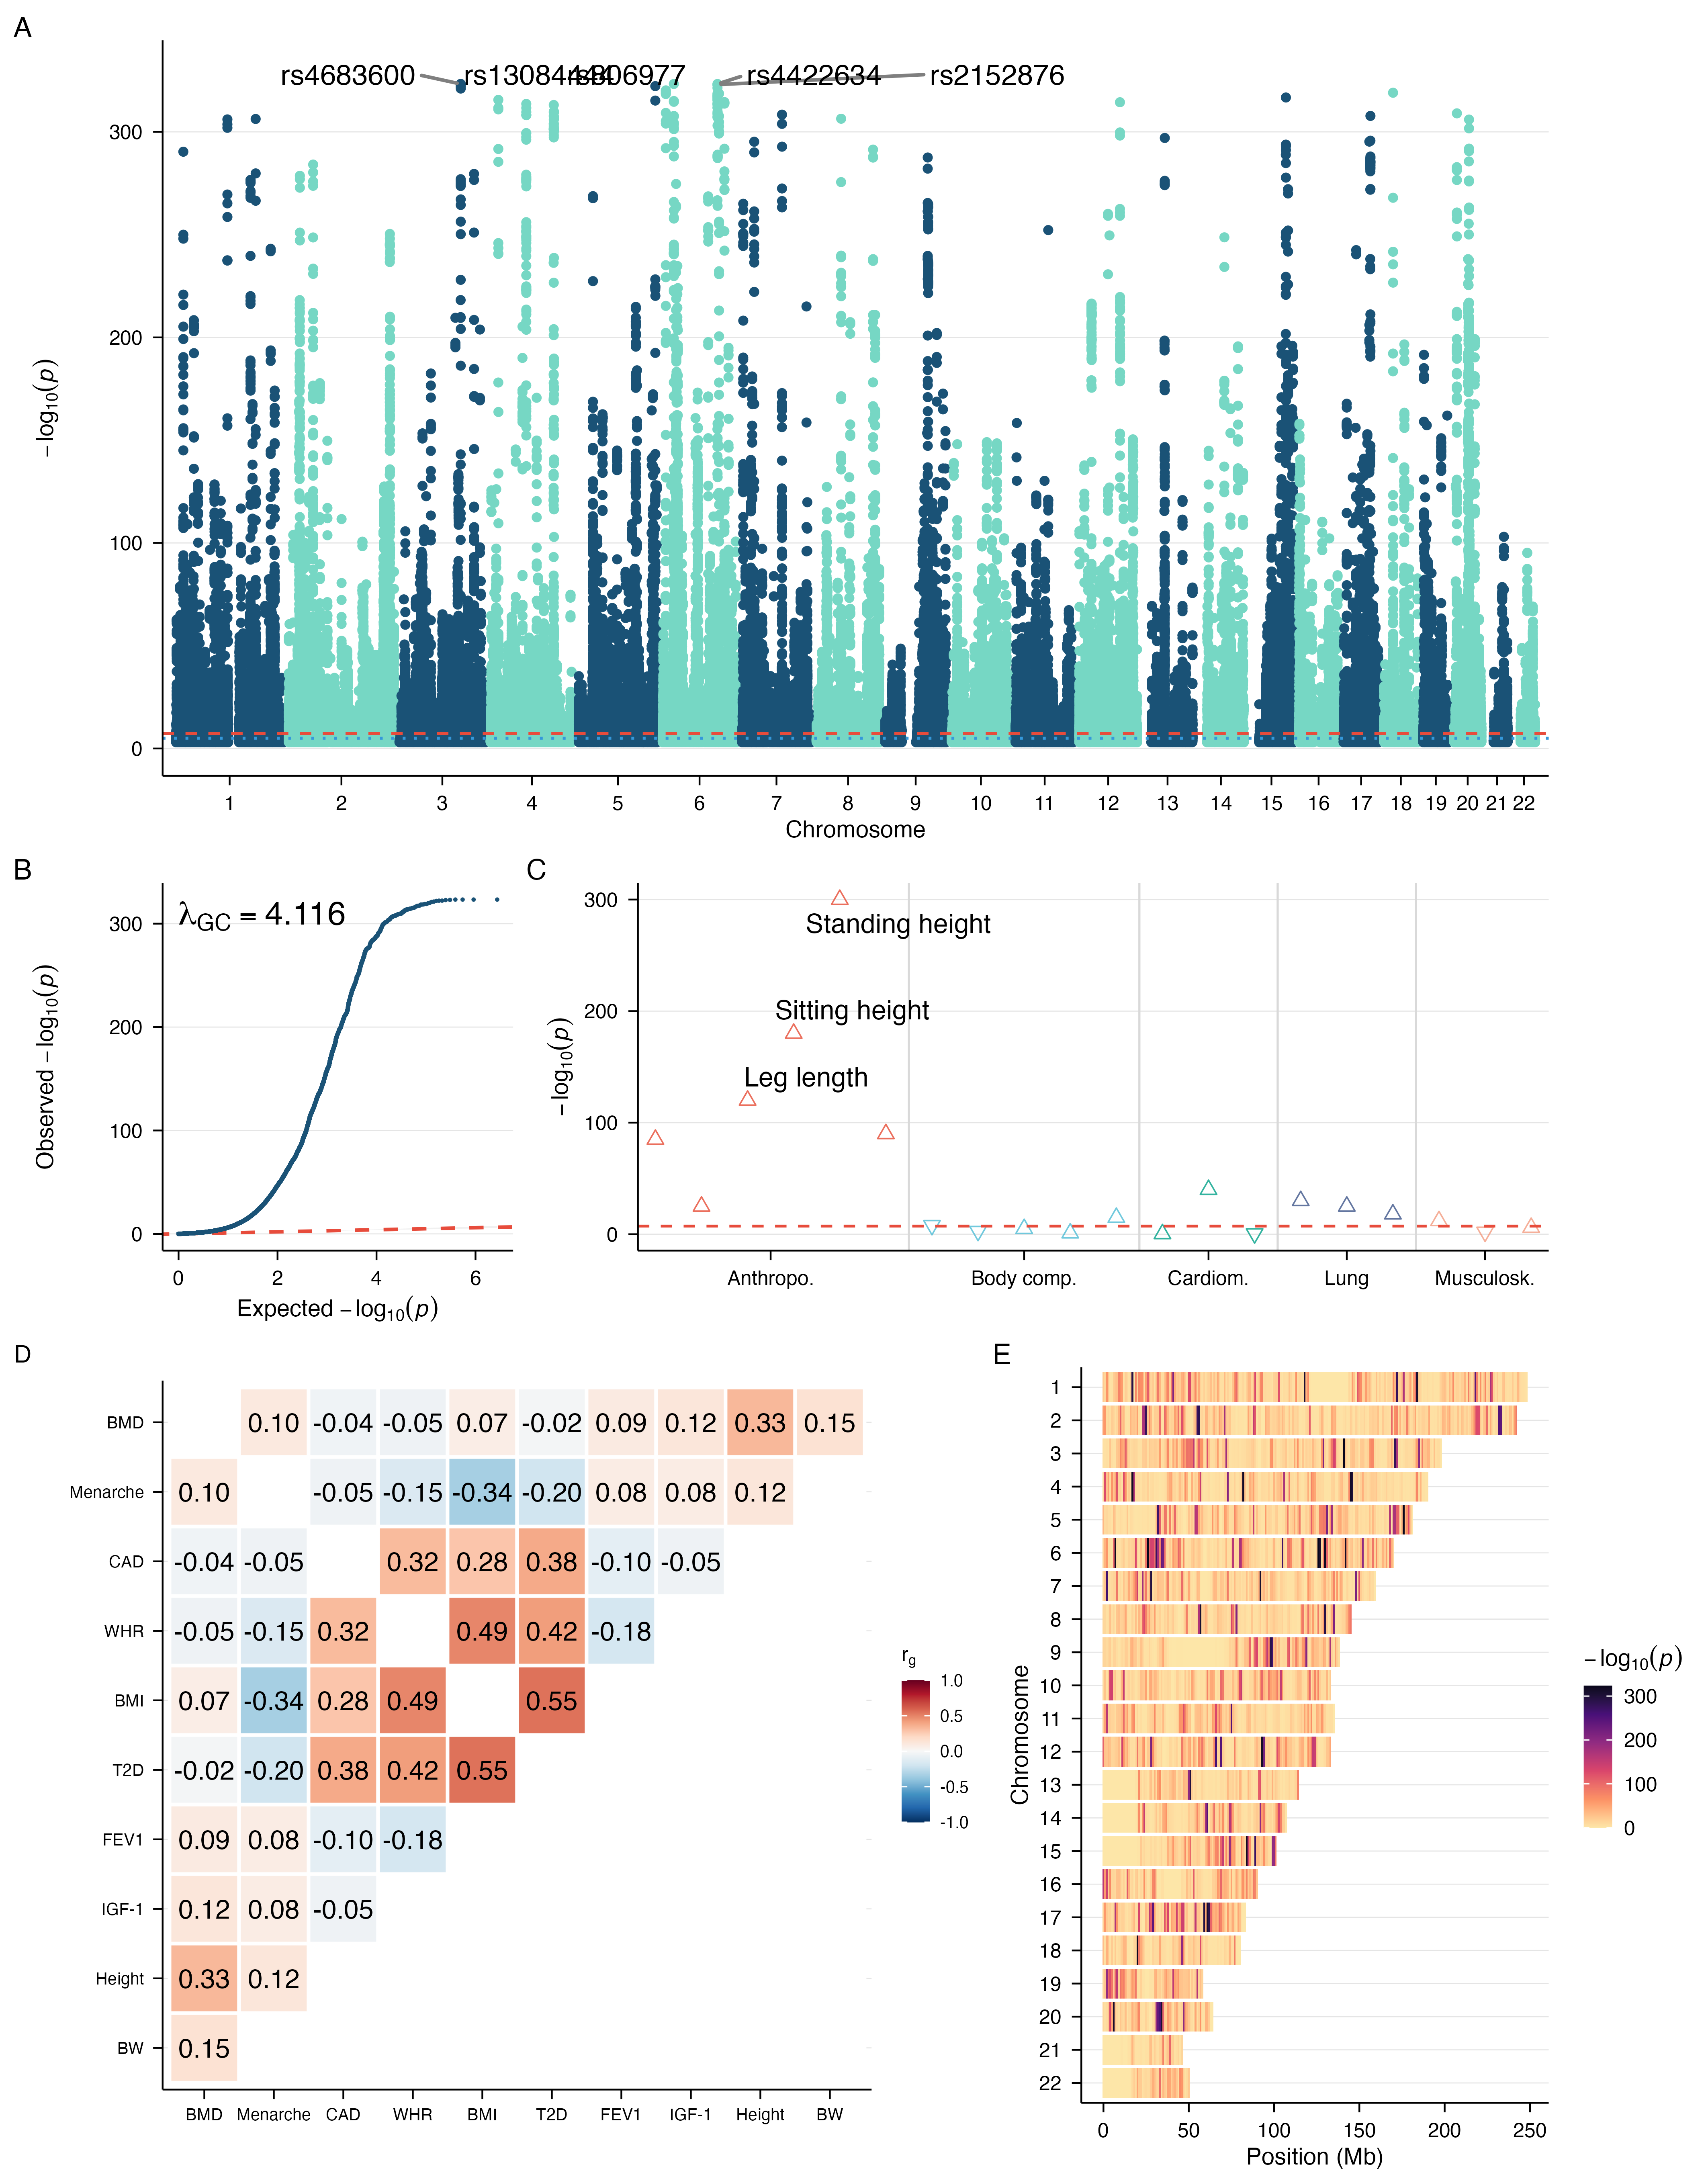
\includegraphics[width=\textwidth]{figures/figure1.png}
\caption{Overview of ggwas visualizations using GIANT consortium height GWAS summary statistics \citep{yengo2022} (1.37M variants, European ancestry). (A)~Manhattan plot with labeled top hits. (B)~QQ plot with 95\% confidence band and $\lambda_{GC}$. (C)~PheWAS plot showing height-associated phenotypes with effect direction triangles. (D)~Genetic correlation matrix (published LD Score regression estimates). (E)~Genome-wide p-value heatmap (darker shading indicates stronger association signal).}\label{fig:overview}
\end{figure*}

\section{Conclusion}

The ggwas package provides a comprehensive, ggplot2-native visualization toolkit for GWAS. By covering the full workflow from quality control through discovery to post-GWAS interpretation, it eliminates the need for ad~hoc plotting scripts. Novel visualizations such as the enrichment Manhattan, genome-wide heatmap, multi-trait overlay, and density--signal dual-track comparison are not available in existing packages. The SNP density karyogram with built-in chromosome data for human, mouse, and cattle---and UCSC integration for any other species---makes the package applicable across organisms. Performance optimizations make ggwas practical for biobank-scale datasets.

\section*{Supplementary Data}

Supplementary Figure~S1 demonstrates all 17 plot types on GIANT height GWAS data: (S1)~Manhattan, (S2)~QQ, (S3)~Miami, (S4)~locus zoom, (S5)~circular Manhattan, (S6)~enrichment Manhattan, (S7)~multi-trait Manhattan, (S8)~genome-wide heatmap, (S9)~effect-size volcano, (S10)~summary dashboard, (S11)~PheWAS, (S12)~colocalization, (S13)~fine-mapping, (S14)~genetic correlation, (S15)~genetic architecture, (S16)~SNP density karyogram, (S17)~density--signal comparison.

\section*{Funding}

This work was not externally funded.

\section*{Conflict of Interest}

The author declares no competing interests.

\bibliographystyle{natbib}

\begin{thebibliography}{20}

\bibitem[Benner {\it et~al.}, 2016]{benner2016}
Benner, C. {\it et~al.} (2016) FINEMAP: efficient variable selection using summary data from genome-wide association studies. \textit{Bioinformatics}, \textbf{32}(10), 1493--1501.

\bibitem[Bulik-Sullivan {\it et~al.}, 2015]{bulik2015}
Bulik-Sullivan, B.K. {\it et~al.} (2015) LD Score regression distinguishes confounding from polygenicity in genome-wide association studies. \textit{Nature Genetics}, \textbf{47}(3), 291--295.

\bibitem[Bycroft {\it et~al.}, 2018]{bycroft2018}
Bycroft, C. {\it et~al.} (2018) The UK Biobank resource with deep phenotyping and genomic data. \textit{Nature}, \textbf{562}(7726), 203--209.

\bibitem[Denny {\it et~al.}, 2013]{denny2013}
Denny, J.C. {\it et~al.} (2013) Systematic comparison of phenome-wide association study of electronic medical record data and genome-wide association study data. \textit{Nature Biotechnology}, \textbf{31}(12), 1102--1111.

\bibitem[{ENCODE Project Consortium}, 2012]{encode2012}
{ENCODE Project Consortium} (2012) An integrated encyclopedia of DNA elements in the human genome. \textit{Nature}, \textbf{489}(7414), 57--74.

\bibitem[Giambartolomei {\it et~al.}, 2014]{giambartolomei2014}
Giambartolomei, C. {\it et~al.} (2014) Bayesian test for colocalisation between pairs of genetic association studies using summary statistics. \textit{PLoS Genetics}, \textbf{10}(5), e1004383.

\bibitem[Kurki {\it et~al.}, 2023]{kurki2023}
Kurki, M.I. {\it et~al.} (2023) FinnGen provides genetic insights into a wide spectrum of diseases. \textit{Nature}, \textbf{613}(7944), 508--518.

\bibitem[Lewis {\it et~al.}, 2025]{lewis2025}
Lewis, M.J. {\it et~al.} (2025) locuszoomr: an R package for publication-ready regional association plots. \textit{Bioinformatics Advances}, \textbf{5}(1), vbaf016.

\bibitem[Mbatchou {\it et~al.}, 2021]{mbatchou2021}
Mbatchou, J. {\it et~al.} (2021) Computationally efficient whole-genome regression for quantitative and binary traits. \textit{Nature Genetics}, \textbf{53}(7), 1097--1103.

\bibitem[Purcell {\it et~al.}, 2007]{purcell2007}
Purcell, S. {\it et~al.} (2007) PLINK: a tool set for whole-genome association and population-based linkage analyses. \textit{American Journal of Human Genetics}, \textbf{81}(3), 559--575.

\bibitem[{Roadmap Epigenomics Consortium}, 2015]{roadmap2015}
{Roadmap Epigenomics Consortium} (2015) Integrative analysis of 111 reference human epigenomes. \textit{Nature}, \textbf{518}(7539), 317--330.

\bibitem[Turner, 2018]{turner2018}
Turner, S.D. (2018) qqman: an R package for visualizing GWAS results using Q-Q and Manhattan plots. \textit{Journal of Open Source Software}, \textbf{3}(25), 731.

\bibitem[Wang {\it et~al.}, 2020]{wang2020}
Wang, G. {\it et~al.} (2020) A simple new approach to variable selection in regression, with application to genetic fine mapping. \textit{Journal of the Royal Statistical Society: Series B}, \textbf{82}(5), 1273--1300.

\bibitem[Wickham, 2016]{wickham2016}
Wickham, H. (2016) \textit{ggplot2: Elegant Graphics for Data Analysis}. Springer-Verlag, New York.

\bibitem[Yengo {\it et~al.}, 2022]{yengo2022}
Yengo, L. {\it et~al.} (2022) A saturated map of common genetic variants associated with human height. \textit{Nature}, \textbf{610}(7933), 704--712.

\bibitem[Yang {\it et~al.}, 2011]{yang2011}
Yang, J. {\it et~al.} (2011) Genomic inflation factors under polygenic inheritance. \textit{European Journal of Human Genetics}, \textbf{19}(7), 807--812.

\bibitem[Yang {\it et~al.}, 2011b]{yang2011gcta}
Yang, J. {\it et~al.} (2011) GCTA: a tool for genome-wide complex trait analysis. \textit{American Journal of Human Genetics}, \textbf{88}(1), 76--82.

\bibitem[Yin, 2024]{yin2024}
Yin, L. (2024) CMplot: Circle Manhattan Plot. R package version 4.5.1. \url{https://CRAN.R-project.org/package=CMplot}.

\bibitem[Zhou and Stephens, 2012]{zhou2012}
Zhou, X. and Stephens, M. (2012) Genome-wide efficient mixed-model analysis for association studies. \textit{Nature Genetics}, \textbf{44}(7), 821--824.

\end{thebibliography}

\end{document}
